\documentclass[../thesis.tex]{subfiles}
\graphicspath{{\subfix{../Afbeeldingen/}}}

\begin{document}
\section{RQa, how do we measure the energy consumption}
\color{red}\textbf{Also notes}\color{black}
[Solution?] Scaphandre
https://github.com/hubblo-org/scaphandre/
measure power consumptoin of tech services and get data in a convenient form
examples can be found here: https://metrics.hubblo.org/d/GOHnbBO7z/scaphandre?orgId=1&refresh=15m

[Solution?] pcm-monitor utility, dont know how to get it working

=========================================================================================================
[Hardware]
https://ieeexplore.ieee.org/stamp/stamp.jsp?tp=&arnumber=9663203
Leia: A Lightweight Cryptographic Neural Network Inference System at the Edge
 10.1109/TIFS.2021.3138611

We implement Leia and deploy it on Raspberry Pi
Usw COOWOO popwer meter COOWOO USB Digital Power Meter Tester. [Online]. Available:
http://www.coowootech.com/tools.html [[HARDWARE]]

------------

[Hardware]
https://ieeexplore.ieee.org/stamp/stamp.jsp?tp=&arnumber=9120239
The voltage and current are measured using a
Powerjive USB multimeter and the power is calculated by the
multiplication of voltage and current

------------

[Java] 
Chiyoung Seo, Sam Malek, and Nenad Medvidovic. “Component-level energy
consumption estimation for distributed java-based software systems”. In: Lecture Notes in Computer Science (including subseries Lecture Notes in Artificial Intelligence and Lecture Notes in Bioinformatics) 5282 LNCS (2008). ISSN:
16113349. DOI: 10.1007/978-3-540-87891-9\_7.

------------

////////// GOOGLE //////////////////
[No open source implementation found]
https://ceur-ws.org/Vol-1938/paper-san.pdf
introduce crapl a c rapl tool, no open soure implementation found

[Solution?]
https://github.com/hubblo-org/scaphandre/
measure power consumptoin of tech services and get data in a convenient form
examples can be found here: https://metrics.hubblo.org/d/GOHnbBO7z/scaphandre?orgId=1&refresh=15m

[Theoretical calculation based on data movement, not actual overhead of program]
https://arxiv.org/pdf/1611.05128.pdf
With the idea of exploiting data reuse in a multi-level memory hierarchy, Chen et al. [21] have presented a framework that can estimate the energy consumption of a CNN for inference
[21] Y. Chen, J. Emer, and V. Sze, “Eyeriss: A Spatial Architecture for Energy-Efficient Dataflow for Convolutional Neural Networks,” in ISCA, 2016.
[22] Y. Chen, T. Krishna, J. Emer, and V. Sze, “Eyeriss: An Energy-Efficient Reconfigurable Accelerator for Deep Convolutional Neural Networks,” in ISSCC, 2016.

[Hardware]
https://dl.acm.org/doi/pdf/10.1145/3310273.3323070

////////// Survey //////////////////
https://dl.acm.org/doi/pdf/10.1145/3141842.3141846
Survey of Approaches for Assessing Software Energy Consumption

[Hardware] Silicon Labs [19] provide an Eclipse-based IDE and development boards for ARM Cortex microcontrollers that allow measuring and profiling the energy consumption of embedded software at runtime. Energy consumption measurements for each method call are provided in a table. This system is commercially available and uses a low-cost development
board with fast current and voltage sensors. The processor’s program counter is read periodically and its value is sent to the host computer along with voltage and current
measurements. The program running on the microcontroller is statically linked, uploaded by the host computer and resides at a previously known and constant address in memory. Hence, the address of the program counter is sufficient to infer the currently executed method.

[Android] Green Droid [3] instruments Android programs and uses PowerTutor [24] to measure their energy consumption at runtime. A trace of the instrumented program and the measured energy consumption are then used to create visualizations in the form of diagrams. These visualizations can help programmers to identify parts of their applications with problematic energy behaviour. To measure energy consumption, PowerTutor relies on a component-based model of the device’s energy usage that can be automatically generated by running a calibration program on the device under test 

[Java] ELens [10] annotates Java source code for Android with energy consumption estimates. An IDE visualizes this by coloring code according to its estimated energy consumption. The estimates are derived from an instruction-level energy consumption model with path dependencies that has been created by the authors for some specific device.  Evaluating this approach with actual energy measurements gives an accuracy error of about 10\% for methods that run longer than 10ms. Methods with a runtime of less than 10ms could not be measured by the setup used by the authors ( https://ieeexplore.ieee.org/stamp/stamp.jsp?tp=&arnumber=6606555 eLens for android applications)

Hardly any implementations found, a lot of approaches. While literature and too lsearch was not performed in a very systematic way
However, we can report that there is a peak of literature on the energy consumption in Android systems. 

//////////// Thesis //////////////////
https://ul.qucosa.de/api/qucosa%3A77194/attachment/ATT-0/
The software scope is chosen because it does not require extra hardware,
e. g. an ampere meter, to take measurements

Measurements can be taken in Joule or Watt. These units can be used interchangeably
when the time frame is known. It is generally advised to use Joule for small and timelimited measurements like the energy usage of a function. Watt is better suited for
longer or indefinitely running program

Power = energy/time

Instant power measurements require extra hardware
Time measurement is based on the drainage of the energy stored in a battery. Laptops are ideally suited for this technique because they are equiped with integrated batery.
Creating model can remove biggest disadvantage: namely the dependency on physical instrumentation. Isolate energy consumption of single application.  

[Java and linux only]
https://github.com/kliu20/jRAPL
Can only measure energy consumption on linux

[Python and not program specific]
https://github.com/powerapi-ng/pyRAPL
calculates global energy consumption of all the processes running on the machine. 

[Linux only]
https://github.com/kentcz/rapl-tools
./AppPowerMeter sleep 5
will measure the total energy and average power of the CPU while it runs "sleep 5". The CPU power is sampled every 100ms then written to rapl.csv.

[not program specific]
https://github.com/sosy-lab/cpu-energy-meter

[Only battery devices]
PowerTOP

[Possible but no documentation]
https://gitlab.com/MarcoCouto/c-lem
\section{Design of experiments}
\section{Explaining testing environment}
\section{Results}

\color{red}\textbf{these are the first results from the experiments, they need a lot of finetuning}\color{black}
\begin{figure}[h!]
    \centering
    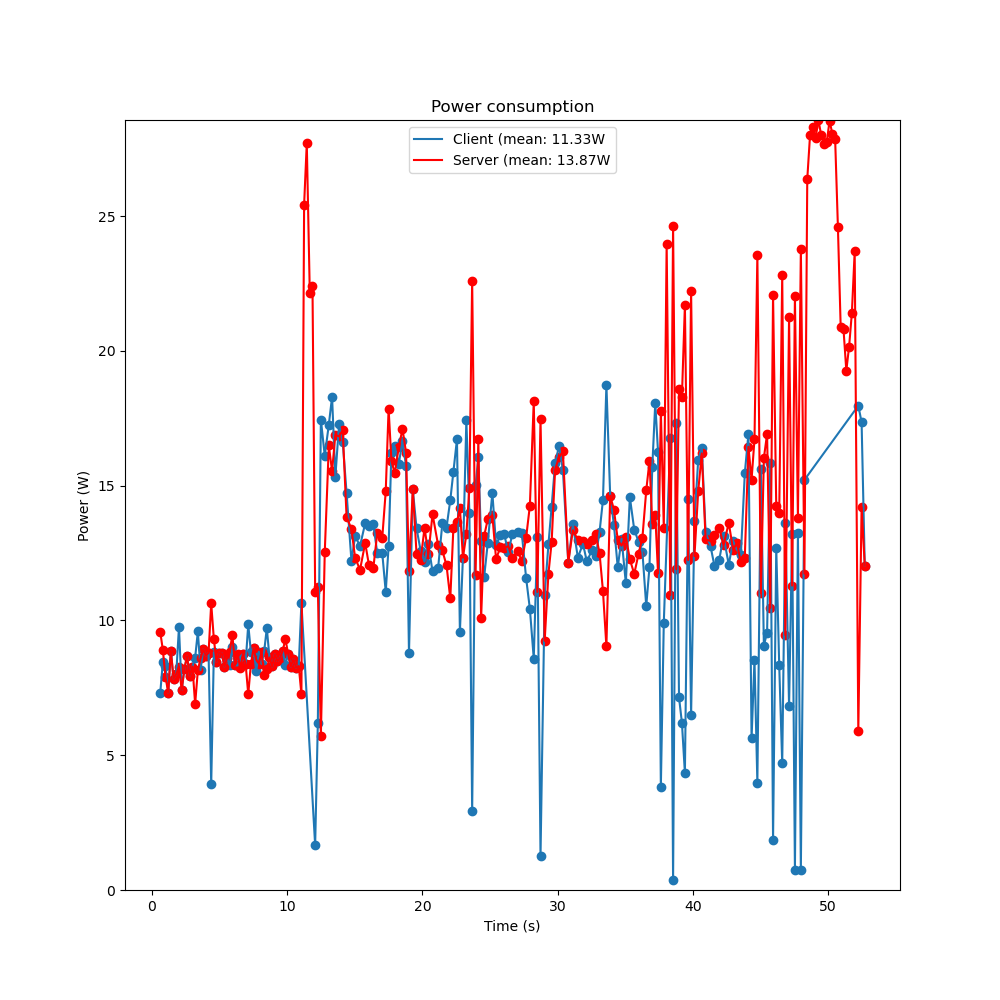
\includegraphics[width=\textwidth,height=\textheight,keepaspectratio]{Thesis/Images/cheetah-sqnet.png}
    \caption{Running the SNNI cheetah on sqnet}
    \label{fig:my_label}
\end{figure}
\newpage
\begin{figure}[h!]
    \centering
    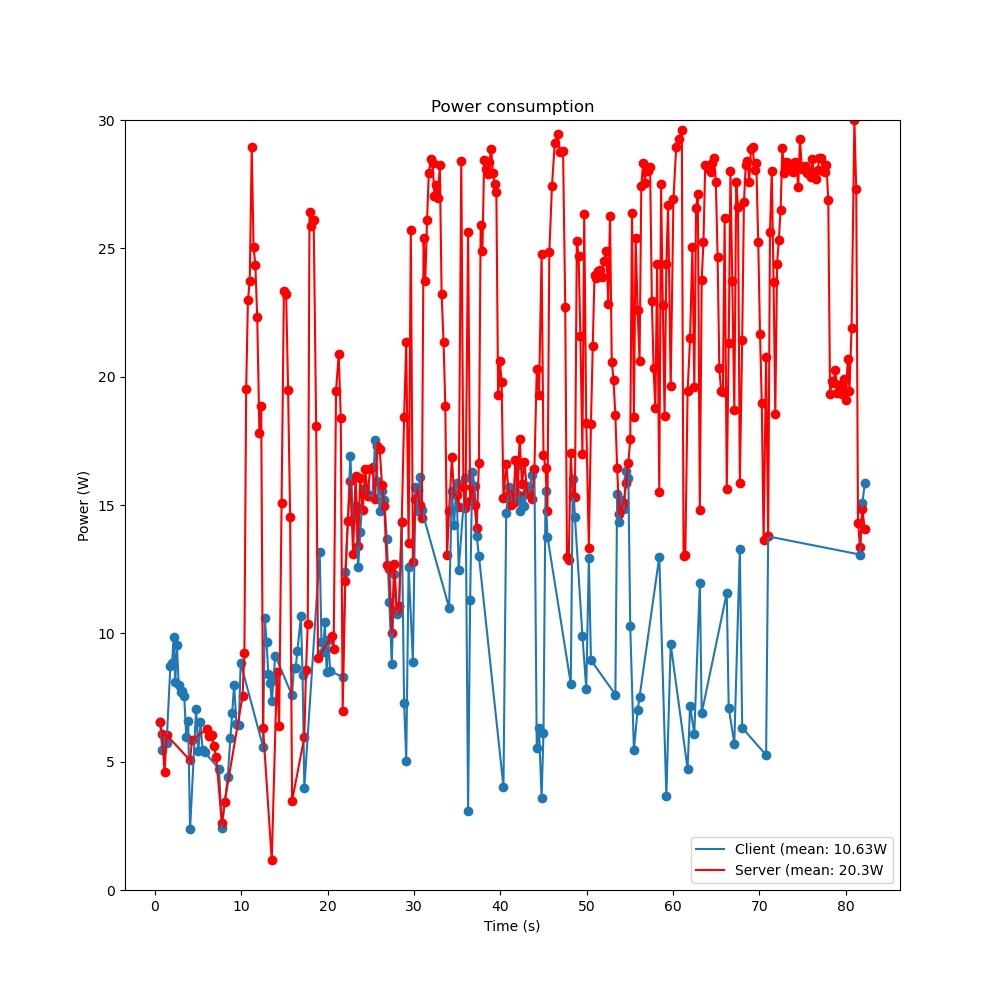
\includegraphics[width=\textwidth,height=\textheight,keepaspectratio]{Thesis/Images/SCI_HE-sqnet.png}
    \caption{Running the SNNI CryptFlow2 on sqnet}
    \label{fig:my_label}
\end{figure}
\section{RQb, what are the differences on server and client side and what are the implications}
\end{document}